\documentclass[12pt]{article}

\usepackage{amsmath} 
\usepackage{graphicx} %package for including images
\usepackage{caption} 
\usepackage{cancel} %package enabling the cancel (cross out) command
\usepackage[a4paper, hmargin=2.5cm, vmargin=2cm]{geometry} 
\usepackage{enumitem} %package for setting list (enumerate, itemize) margins

\graphicspath{ {../graphics/} } %setting image folder path
\setlist[enumerate]{leftmargin=0mm, itemsep=20pt} %setting enumerate list properties like margin

\title{Probability for the Enthusiastic Beginner}
\author{David Morin}
\date{}

\begin{document}
\maketitle

\begin{enumerate}

\item 
Factorial of $N$, denoted $N!$, is the product of the first $N$ positive integers, namely $(1)(2)(3)\dots(N-1)(N)$.
$0!$ is defined to be $1$. 

\item 
Permutation of a set of objects refers to a particular way of ordering them (ie. ordered arrangement). \\
If the set is $ \{ A B C \}$, then $ \{C A B \} $ is a permutation as is $ \{B A C\} $.
\\\\
The number of possible permutations for a set of $N$ items is $N!$. It can be induced from the simplest cases where permutations are counted.
\\\\
For $N=1$, $P_1$ is apparently $1$. 
\\\\
For $N=2$, we have $(1, 2), (2, 1)$, so $P_2 = 2 = 2!$
\\\\
For $N=3$, we have $P_3 = 6$,

{
\centering
\begin{tabular}{c c c}
    
    (1,2,3) & (2,1,3) & (3,1,2) \\
    (1,3,2) & (2,3,1) & (3,2,1)
    
\end{tabular} \par
}

Note that the permutations are grouped into 3 subgroups by iterating through the objects and fixing each to the first position. For the subgroup having 3 fixed in the first position, the permutations of the remaining positions are identical to $P_2$. As the objects are merely nominal,
this holds for all subgroups, so $P_3 = (3)(P_2) = (3)(2!) = 3 \cdot 2 = 3! = 6$.
\\\\
For $N=4$, we have $P_4 = 24$, 

{
\centering
\begin{tabular}{c c c c}
    
    (1,2,3,4) & (2,1,3,4) & (3,1,2,4) & (4,1,2,3) \\
    (1,2,4,3) & (2,1,4,3) & (3,1,4,2) & (4,1,3,2) \\
    (1,3,2,4) & (2,3,1,4) & (3,2,1,4) & (4,2,1,3) \\
    (1,3,4,2) & (2,3,4,1) & (3,2,4,1) & (4,2,3,1) \\ 
    (1,4,2,3) & (2,4,1,3) & (3,4,1,2) & (4,3,1,2) \\
    (1,4,3,2) & (2,4,3,1) & (3,4,2,1) & (4,3,2,1) 
    
\end{tabular} \par
}

Again, we have 4 subgroups, each having 6 permutations; we see that in the subgroup having 4 fixed in first position, the remaining permutations are identical to $P_3$.
As a result, $P_4 = (4)(P_3) = (4)(3!) = 4 \cdot 6 = 24$.
\\\\
By induction, we see that $P_N = N \cdot P_{N-1}= N \cdot (N-1)! = N! $. 

\item 
For ordered sets of $n$ objects selected from $N$ distinct objects where repetitions allowed (equivalently, \textbf{with replacements}), the number of possible arrangements is $N^n$. 
For example, number of possible outcomes in rolling a fair dice 3 times is $6 \cdot 6 \cdot 6 = 6^3 = 216$.
\\\\
For ordered sets of $n$ objects chosen from $N$ distinct objects where repetitions not allowed (equivalently, \textbf{without replacements}), the number of possible arrangements is 
$_N P_n = N(N-1)(N-2)\dots (N-(n-1)) $. The last factor is $N-(n-1)$ because at $n^{th}$ selection, $n-1$ items have already been chosen so only $ N - (n-1)$ remain free. 
$_N P_n$ can be simplified to $ _N P_n = N(N-1)(N-2) \dots (N-n+1) \cdot \frac{(N-n)!}{(N-n)!} = \frac{N!}{(N-n)!}$.
\\\\
Apparently, if $ n = N$, $_N P_n = \frac{N!}{0!} = N!$


\item 
Now instead of ordered sets where $AB \neq BA$, we turn to unordered sets where the order or sequence in the set is not important so $AB = BA$. 
The number of possible unordered arrangements in picking $n$ out of $N$ distinct objects \textbf{without replacements} is denoted by $_N C_n$ or $\binom{N}{n}$.
\\\\
We know there are $_N P_n$ ordered arrangements in picking $n$ out of $N$ distinct objects and that there are $n!$ ways in arranging those $n$ objects, which result in overcounting when order is not important and so must be discounted. 
Thus, the number of unordered possible outcomes is 
$$
_N C_n = \binom{N}{n} = \frac{_N P_n}{n!} = \frac{N!}{(N-n)!(n!)}
$$
Note that $\binom{N}{n_1} = \binom{N}{n_2}$ if $ n_1 + n_2 = N$; for example, $\binom{10}{4} = \frac{10!}{6!4!} = \binom{10}{6} = \frac{10!}{4!6!}$.
Intuitively, when we pick $n$ out of $N$ items (say into a box), we are basically generating two sets of objects, the picked $n$ (in the box) and unpicked $N-n$ (out of the box). Those two sets are complementary so the number of ways in generating one is equal to that in generating the other.


\item 
The number of possible \textbf{unordered} arrangements (order not important) in picking $n$ out of $N$ distinct objects \textbf{with replacement} is not as commonly encountered as $_N P_n$ and $_N C_n$, both are \textbf{without replacement}.
\\\\
The problem is frequently approached by restating it into something called \textit{stars and bars}. The restated problem is essentially equivalent to the original one but has a simpler form.
Because order is not important in the set, the selected items can be sorted by some order (alphabet or value, ascending or descending) on a line. 
For example, if we pick from $3$ objects (say $\{A,B,C\}$) $6$ times with replacement, some potential (sorted) outcomes are: 
\begin{center}
\underline{A} \quad \underline{A} \quad \underline{B} \quad \underline{B} \quad \underline{C} \quad \underline{C}   
\\
\underline{B} \quad \underline{B} \quad \underline{B} \quad \underline{C} \quad \underline{C} \quad \underline{C}
\\
\underline{B} \quad \underline{B} \quad \underline{B} \quad \underline{B} \quad \underline{B} \quad \underline{B}
\\
\underline{A} \quad \underline{A} \quad \underline{A} \quad \underline{A} \quad \underline{A} \quad \underline{C}
\end{center}

Once aggregated, the items can all be generically denoted by $\star$, and the change of value indicated by $\Delta$. Thus, there are $n$ $\star$ and $(N-1) \ \Delta$.
There are now $n + (N - 1)$ \textit{slots} to fill in this representation.
The above outcomes can be alternatively represented as:
\begin{center}
    \underline{$\star$} \quad \underline{$\star$} \quad \underline{$\Delta$} \quad \underline{$\star$} \quad \underline{$\star$} \quad \underline{$\Delta$} \quad \underline{$\star$} \quad \underline{$\star$}   
    \\
    \underline{$\Delta$} \quad \underline{$\star$} \quad \underline{$\star$} \quad \underline{$\star$} \quad \underline{$\Delta$} \quad \underline{$\star$} \quad \underline{$\star$} \quad \underline{$\star$} 
    \\
    \underline{$\Delta$} \quad \underline{$\star$} \quad \underline{$\star$} \quad \underline{$\star$} \quad \underline{$\star$} \quad \underline{$\star$} \quad \underline{$\star$} \quad \underline{$\Delta$}     
    \\
    \underline{$\star$} \quad \underline{$\star$} \quad \underline{$\star$} \quad \underline{$\star$} \quad \underline{$\star$} \quad \underline{$\Delta$} \quad \underline{$\Delta$} \quad \underline{$\star$}   
\end{center}
Each way to place those $N-1$ $\Delta$ in the $n + N -1$ \textit{slots} represents a unique unordered arrangement of $n$ items out of $N$.
Thus, the number of ways that the $\Delta$ can be arranged is equivalent to the number of ways that $n$ items can be chosen from $N$ when order is not important and with replacement.
\\\\
That number is equal to 
$$
_{(n + N - 1)} C_{(N - 1)} \quad \text{or} \quad \binom{n + N - 1}{N - 1} = \binom{n + N -1}{n}
$$

\item
A basic binomial property is:
$$
\binom{n}{k} = \binom{n-1}{k-1} + \binom{n-1}{k}
$$
This can be understood intuitively by thinking there is a specific item in $n$ that is marked, so the number of unordered ways in picking $k$ out of $n$ without replacement is equal to
the sum of the case where the marked item is included and the case where the marked item is not included. If included, there will be $k-1$ items to select out of $n-1$; if not included, there will be $k$ items to select out of $n-1$.
\\\\
Algebraically, 
\begin{align*}
\binom{n-1}{k-1} & = \frac{(n-1)!}{(n-1-k+1)!(k-1)!} = \frac{(n-1)!}{(n-k)!(k-1)!} 
\\
\binom{n-1}{k} & = \frac{(n-1)!}{(n-1-k)!k!}
\end{align*}
The common denominator in these two fractions is $(n-k)!(k)!$, so multiply by $\frac{k}{k}$ and $\frac{n-k}{n-k}$.
\begin{align*}
\binom{n-1}{k-1} + \binom{n-1}{k} & = \frac{(n-1)!}{(n-k)!(k-1)!} \cdot \frac{k}{k} + \frac{(n-1)!}{(n-1-k)!k!} \cdot \frac{n-k}{n-k} \\
& = \frac{(n-1)!\cdot k}{(n-k)! \cdot k!} + \frac{(n-1)! \cdot (n-k)}{(n-k)! \cdot k!}  \\
& = \frac{(n-1)! \cdot (k + (n-k))}{(n-k)! \cdot k!} \\
& = \frac{(n-1)! \cdot n}{(n-k)! \cdot k!} = \frac{n!}{(n-k)! \cdot k!} = \binom{n}{k} 
\end{align*}

\item
For two events $A$ and $B$, the probability that both events occur is called joint probability, denoted by $P(A \cap B)$. When analysing multiple events, it is important to know if the events are independent or dependent. 
Two events are independent if the occurrence (or nonoccurrence) of one does not change the probability of occurrence of the other. In Venn diagram, independent events $A, B$ are in two different sample spaces $S_1, S_2$. If $A$ and $B$ are independent, 
$$
P(A \text{ and } B) = P(A \cap B) = P(A) \cdot P(B)
$$
Since $0 \leq p \leq 1$, we see that $P(A \cap B)$ must be lower than (or equal to) $P(A)$ and $P(B)$. Joint probability can be viewed alternatively by 
imagining a 2-dimensional plane having a horizontal line and vertical line of lengths 1 each, so area is also 1. P(A) has width $w$ on the horizonal line and P(B) has height $h$ on the vertical line.  
$P(A \cap B)$ is represented by the region where $w$ and $h$ intersect over the entire square. Even if $P(B) = h = 1$, the intersecting region gives $P(A \cap B) = w = P(A)$. For $h < 1$, the region becomes smaller and so $P(A \cap B) < P(A)$; in the extreme case where $h = 0$, the region is nil and so $P(A \cap B) = 0$.
Thus, the addition of any new event $B$ will be like placing a restriction on event $A$, resulting in joint probability always lower than (at most equal to) the individual probabilities.

\item
When $A$ and $B$ are independent, $P(A | B) = P(A)$ and $P(B|A) = P(B)$. Independence is symmetrical (there is no direction), so $B$ being independent of $A$ implies $A$ being independent of $B$.
Thus, $P(A | B) = P(A) \implies P(B|A) = P(B)$.

\item 
Two events are dependent if the occurrence (or nonoccurrence) of one changes the probability of occurrence of the other. A simple example is where $A$ is the event of storm and $B$ is the event of hiking; obviously $P(B)$ changes on the occurrence of $A$.
Not only that given there was a storm, the probability of Sally having gone hiking is different from the unconditional probability $P(B|A) \neq P(B)$, but also that knowing Sally had gone hiking, the probability that a storm occurred is different from its unconditional probability $P(A|B) \neq P(A)$.
\\\\
In Venn diagram, $P(A)$ and $P(B)$ are the relative sizes of their respective event spaces $A, B$ in the sample space $S$, and $P(A \cap B)$ is the size of their intersection (overlap) in $S$. 
Thus, when event $B$ has occurred, the sample space must now adjust (shrink) from $S$ to $B$; the probability of $A$ therefore becomes its relative event size within $B, A \cap B$.
$$
P(A|B) = \frac{P(A \cap B)}{P(B)}
$$
From another perspective, let $A_1, A_2$ be a sequence of events where $A_1$ occurs first, 
$$
P(A_2 | A_1) = \frac{P(A_1 \cap A_2)}{P(A_1)} \quad \text{or} \quad P(A_1 \cap A_2) = P(A_1) \cdot P(A_2 | A_1)
$$

\item
Two events are exclusive if they cannot both happen such that occurrence of one precludes the occurrence of the other. 
In Venn diagram, two exclusive events are two event spaces in the sample space having no intersecting region. 
Given they are impossible to occur together, $P(A \cap B) = 0$. 
We can however think about the probability of either $A$ or $B$ occurring which is sum of their individual probabilities or sum of event spaces $A$ and $B$ in $S$, namely $P(A \cup B) = P(A) + P(B)$.
\\\\
Because event $A$ and its complement, denoted $A^c$ or $A'$, are by definition exclusive, $P(A \cup A^c) = P(A) + P(A^c) = P(S) = 1$.
\\\\
When events $A$ and $B$ are not exclusive, summing their event spaces will double count the intersecting region, $A \cap B$, which belongs to both $A$ and $B$ so has to be subtracted out. 
Thus, $P(A \cup B) = P(A) + P(B) - P(A \cap B)$.
\\\\
It gets more complicated for more events, but the concept is to track the overlapping regions and adjust for them in the calculation.


\item
\textbf{The Monty Hall problem} \\
The so-called Monty Hall question is seemingly simple but involes some mental excercise and demonstrates well the value of new information.
\\\\
The setup is that there are three doors where a prize is behind one and trash bins behind two; the guest is to pick the door containing the prize. The host, who knows what's behind each door, will intentionally open one of the two unpicked doors to reveal the trash bin. 
The guest is then offered the chance to stay with the originally picked door or switch to the other unopened door. The question is whether it is beneficial to switch or stay.

\begin{table}[h]
\centering
\begin{tabular}{ p{0.3\linewidth} c p{0.4\linewidth} }
\raisebox{-0.8\totalheight}{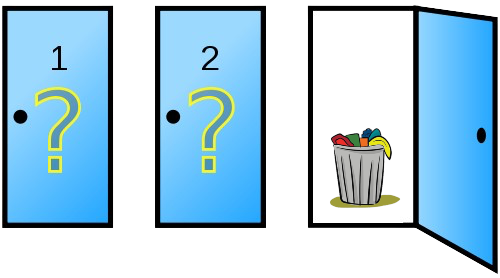
\includegraphics[width=\linewidth]{monty hall doors}}
& \quad &
\footnotesize{If the guest picks door 1, the host will then open door 3 to intentionally reveal the trash. Should the guest switch to door 2 or stay with door 1?}
\end{tabular}
\end{table}
    
The probability of initially picking the prize, $P(\text{first})$, obviously was $\frac{1}{3}$ and after the purposeful revealation there are two doors left.
The key point is whether the intentional revealation changes $P(\text{first})$ or not; if it does not, that is $P(\text{stay}) = P(\text{first}) = \frac{1}{3}$, then it is beneficial to switch because $P(\text{stay}) + P(\text{stay}^C) = P(\text{stay}) + P(\text{switch}) = 1 \implies P(\text{switch}) = 1 - P(\text{stay}) = 1 - \frac{1}{3} = \frac{2}{3}$.
However, if the revealation does change $ P(\text{first}) = P(\text{stay}) $ to $\frac{1}{2}$, then $ P(\text{stay}) + P(\text{switch}) = 1 \implies P(\text{stay}) = P(\text{switch}) = \frac{1}{2}$, so it is indifferent. If somehow the revealation increased $P(\text{first})$ to over $\frac{1}{2}$, then $P(\text{switch}) < \frac{1}{2}$ and it would be beneficial staying, but there is hardly any logic for this case.
Even one trash door is subsequently removed, that does not change the fact that the initial door was chosen out of three doors, so $P(\text{first})$ remains $\frac{1}{3}$ and $P(\text{stay})$ is also $\frac{1}{3}$. It is therefore beneficial to switch. 
\\\\
Another way of reasoning is whether the host's action of opening a trash door conveys valuable information (recall he has perfect information and guest is uninformed); if so, whether the information can be consumed by staying or switching. 
The action does reveal valuable information because the host knows which one of the two remaining doors contains trash and purposefully opens it and the guest is informed of the rule in advance. This tilts the information asymmetry. The only way to use the information is to switch, so switching shall be logically beneficial.   
\\\\
In terms of permutations, there are $\binom{3}{2} \cdot \binom{1}{1} = 3$ possible arrangements: $\{PTT\}, \{TPT\}, \{TTP\}$, where $P, T$ denote prize and trash.
Without loss of generality, assume the guest picks the first door; in case of $\{PTT\}$, the host can open either the second or third door, $\{P\cancel{T}T\}$ or $\{PT\cancel{T}\}$, and the guest wins by staying or loses by switching. 
\\\\
\begin{tabular}{ | c | c | c | c | c | }
\hline 
\textbf{Probability} & \textbf{Initial Permutation} & \textbf{Modified Permutation} & \textbf{Staying} & \textbf{Switching} \\
\hline
$\frac{1}{3}$ & \{PTT\} & \{P\cancel{T}T\} or \{PT\cancel{T}\} & Win & Lose \\
$\frac{1}{3}$  & \{TPT\} & \{TP\cancel{T}\} & Lose & Win \\
$\frac{1}{3}$ & \{TTP\} & \{T\cancel{T}P\} & Lose & Win \\
\hline
\end{tabular}
\\\\
Staying can only win in one case, where the prize is correctly picked initially, while switching can win in two cases, where the prize is not picked initially. 
This is due to the rule of the game, which flips initial win and loss around by switching. 
The underlying logic manifests if we imagine $100$ doors and the host subsequently eliminates $98$ of them.
\\\\
If Tony enters \textit{after} the trash door is removed, all he knows is the prize is behind one of the two doors, not even which door is originally picked. 
From his perspective, the probability is $\frac{1}{2}$, and so if asked which door is better, his advice should be indifferent. 
Probability differs between them because they have different level of information (guest is partially informed and Tony uninformed), so their optimal choices differ.


\item 
Conditional probability can be restated as 
\begin{align*}
P(A | Z) & = \frac{P(A \cap Z)}{P(Z)} = \frac{P( A \cap Z)}{P( A \cap Z) + P( A^C \cap Z)} \\
 & = \frac{P(A) \cdot P(Z | A)}{P(A) \cdot P(Z | A) + P(A^C) \cdot P(Z | A^C)}  
\end{align*}
If events $A_i$ are mutually exclusive such that $P(A_i \cap A_j) = 0$ for all $i \neq j$ and complete such that $\sum_i A_i = S$, their probabilities conditional on an event $Z$ is 
$$
P(A_k | Z)  = \frac{P(A_k) \cdot P(Z | A_k)}{\sum_i P(A_i) \cdot P(Z | A_i)} \qquad \text{\footnotesize{Bayes formula}}
$$
While the formula is simply a rearrangement of conditional probability, the form it is restated and applied is useful. 

\item 
A random variable is a variable $X$ that can take on different numerical values with certain probabilities, which forms its probability distribution. 
An expected value is the average it should have in a large number of trials and it is a weighted average of its values with probabilities being the weights. 
$$
E(X) = p_1 \cdot x_1 + p_2 \cdot x_2 + \ldots + p_n \cdot x_n = \sum_i p_i \cdot x_i
$$
Also, expected value of a sum is equal to the sums of the individual expected values. It holds regardless of independence. 
\begin{align*}
E(X + Y) & = E(X) + E(Y) \\
E(a_1 X_1 + a_2 X_2 + \ldots + a_n X_n) & = a_1 E(X_1) + a_2 E(X_2) + \ldots + a_n E(X_n)
\end{align*}
For products of random variables, dependency is important. 
$$ 
E(XY) = E(X) \cdot E(Y)  \qquad \text{valid only on \underline{independent} r.v.}
$$
Proof: 
\begin{align*} 
E(XY) & = \sum_{i = 1}^{n_x} \sum_{j = 1}^{n_y} P(x_i, y_j) \cdot x_i y_j \\
& = \sum_{i = 1}^{n_x} \sum_{j = 1}^{n_y} P(x_i) P(y_j) \cdot x_i y_j \qquad \text{\footnotesize{independence assumption}}   \\
& = \left( \sum_{i = 1}^{n_x} P(x_i) \cdot x_i \right) \left( \sum_{j = 1}^{n_y} P(y_j) \cdot y_j \right) 
= E(X) \cdot E(Y)
\end{align*}


\item 
Variance of a random variable $X$ is the expected value of the square of the difference between $X$ and its mean. 
It basically measures how spread out are the possible outcomes of $X$ from its expected value. 
$$
\text{Var}(X) = \sigma_x^2 = E[ (X - \mu)^2 ]
$$

Some basic properties: 
\begin{align*} 
& \text{Var}(a X) = a^2 \text{Var}(X)  \\
& \text{Var}(X + Y) = \text{Var}(X) + \text{Var}(Y) \qquad \text{iff \underline{independent}} 
\end{align*}

Proof: 
\begin{align*} 
\text{Var}(a X) & = E[ \left( (aX) - (a \mu) \right) ^2]  \\
& = E[ (a(x - \mu))^2] \\
& = E[a^2 (x- \mu)^2] \\
& = a^2 E[(x - \mu)^2] = a^2 \text{Var}(X) \\\\
\text{Var} (X + Y)  & = E[ \left( (X+Y) - (\mu_x + \mu_y) \right) ^2] \\ 
& = E[\left( (X - \mu_x) + (Y - \mu_y) \right) ^2] \\ 
& = E[ (X - \mu_x)^2] + 2 \cdot E[(X - \mu_x)(Y - \mu_y)] + E[(Y - \mu_y)^2] \\ 
& = E[ (X - \mu_x)^2] + 2 \cdot 0 + E[(Y - \mu_y)^2] \qquad \text{based on independence} \\
& = \text{Var}(X) + \text{Var}(Y)
\end{align*}
$ E[(X - \mu_x)(Y - \mu_y)] = 0 $ because of $E(XY) = E(X) \cdot E(Y)$ iff $X, Y$ are independent, such that $ E[(X - \mu_x)(Y - \mu_y)] = E(X - \mu_x) \cdot E(Y - \mu_y) = 0 \cdot 0 $.
 











\end{enumerate}

\end{document}
